\documentclass{article}
%% This is the preamble
    \usepackage[utf8]{inputenc}
    \usepackage[dvipsnames,svgnames,x11names,table]{xcolor}
    %% To customize page margins, use geometry
    \usepackage{geometry}
    \geometry{top=1.5in,left=1in, right=1in, bottom = 1.5in}
    %% physics and math packages
    \usepackage{amsmath,derivative,siunitx}
    %% some helpful packages to make internal links in your document
    \usepackage{hyperref}
    %% to include pictures and plots
    \usepackage{graphicx}
    % extra packages for Quantum
    \usepackage{braket}
    \renewcommand{\doteq}{\,\dot{=}\,}


\title{Homework 3}
\author{Adrian deCola}
\date{March 2, 2023}


%% Now we begin the formal document
\begin{document}

\maketitle


\section*{Problem 8.27}
\verb+Problem+: At time $t_0$ a comet is observed at radius $r_0$ traveling with speed $v_0$ at an acute angle $\alpha$ to the line from the comet to the sun. Put the sun at the origin $\mathcal{O}$, with the comet on the $x$ axis (at $t_0$) and its orbit in the $xy$ plane, and then show how you could calculate the parameters of the orbital equation in the form $r = \frac{c}{1 + \epsilon cos(\phi - \delta )}$. Do so for the case that $r_0= 1.0 * 10^{11}m$, $v_0= 45 \frac{km}{s}$, and $\alpha = 50$ degrees. [The sun's mass is about $2.0 * 10^{30}kg$, and $G = 6.7 * 10^{-11} \frac{N*m^2}{kg^2}$.]


\begin{figure}[!h]
    \centering
    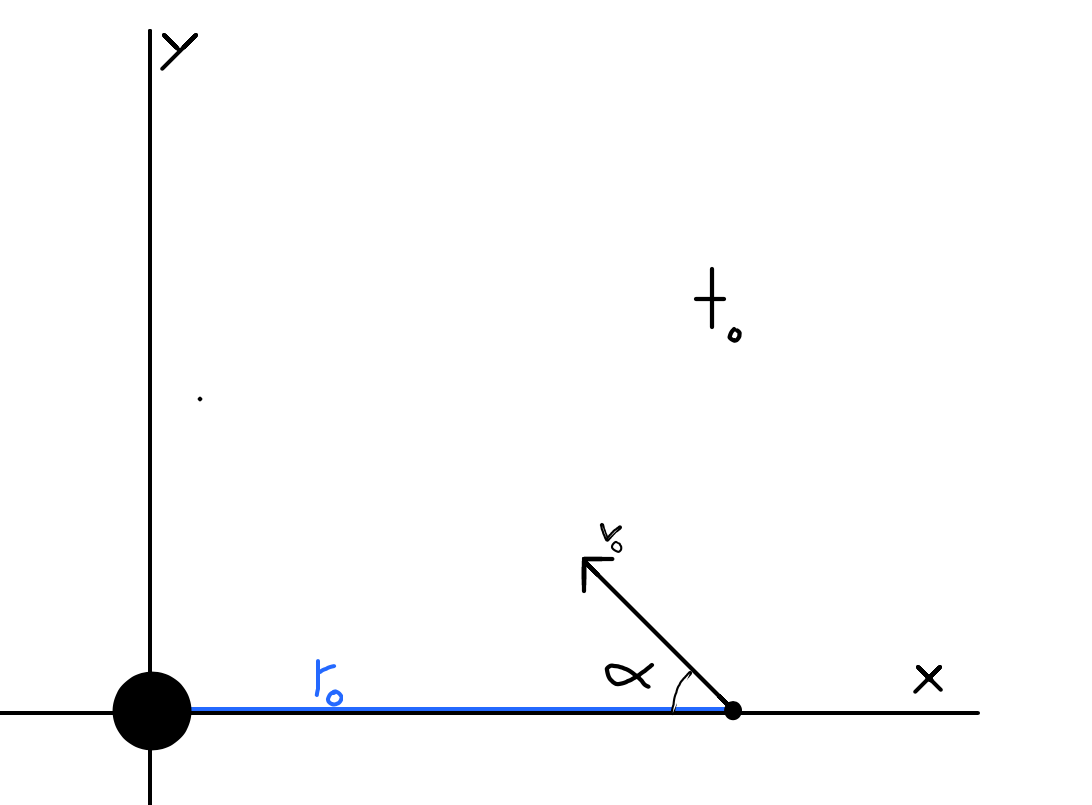
\includegraphics[width=.6\textwidth]{Drawing.png}
    \caption{An illustration of the comet and sun at time $t_0$.}
\end{figure}

\hrule
         \ \ \ 

We want to find the parameters $c$, $\epsilon$, and $\delta$ so that we can know the comet's path in the form 
$$r(\phi) = \frac{c}{1 + \epsilon  cos(\phi - \delta )}$$

We know that $c$, which has units of length, has the following form, $$c = \frac{l^2}{\gamma \mu}$$
where $l$ is the angular momentum, $\gamma$ is the force constant, and $\mu$ is the reduced mass.

Since the inverse-squared force is gravity in this problem:
$$ \gamma = G m_s m_c$$
where $m_s$ is the mass of the sun and $m_c$ is the mass of the comet. Also, since the mass of the sun is so much larger than the mass of the comet, the reduced mass is essentially the mass of the comet, 
$$\mu = \frac{m_cm_s}{m_s + m_c} \approx m_c$$
Since angular momentum is conserved, we get an expression for the angular momentum from the stated parameters at time $t_0$:
$$l=r\times p=r_0 \times p_0 = r_0 \times (m_cv_0)=m_cr_0v_0sin(\pi - \alpha) = m_cr_0v_0sin(\alpha)$$
We can use these to calculate the constant $c$:
\begin{align*}
    c &= \frac{(m_c r_0v_0sin(\alpha))^2}{(G m_s m_c)(m_c)} \\
    c &= \frac{m_c^2 r_0^2 v_0^2 sin^2(\alpha)}{G m_s m_c^2} \\
    c &= \frac{r_0^2 v_0^2 sin^2(\alpha)}{G m_s } \\
\end{align*}
We can use this to solve for $c$ using the known $r_0$, $v_0$, $\alpha$,  $m_s$, and $G$:
$$\boxed{c = \frac{r_0^2 v_0^2 sin^2(\alpha)}{G m_s } }$$
$$\boxed{c = 8.868*10^{10}m}$$
We know that the eccentricity is related to the energy of the comet. 
$$E = T_c + U = \frac{\gamma^2 \mu}{2l^2}(\epsilon^2 - 1) $$
We can calculate the energy at time $t_0$. It is clear that the kinetic energy of the comet is $\frac{1}{2}m_cv_0^2$. Also, the only potential energy is the gravitational potential energy of the comet: $U = -\frac{Gm_sm_c}{r_0}$. Using this we can solve for the eccentricity. 
\begin{align*}
    T_c + U &= \frac{\gamma^2 \mu}{2l^2}(\epsilon^2 - 1) \\
    \frac{1}{2}m_cv_0^2 - \frac{Gm_sm_c}{r_0}&= \frac{(Gm_sm_c)^2 m_c}{2m_c^2 r_0^2 v_0^2 sin^2(\alpha)}(\epsilon^2 - 1)\\
    \frac{1}{2}m_cv_0^2 - \frac{Gm_sm_c}{r_0}&= \frac{G^2m_s^2 m_c}{2r_0^2 v_0^2 sin^2(\alpha)}(\epsilon^2 - 1)\\
    \frac{1}{2}v_0^2 - \frac{Gm_s}{r_0}&= \frac{G^2m_s^2}{2r_0^2 v_0^2 sin^2(\alpha)}(\epsilon^2 - 1)\\
    \epsilon^2 - 1 &= \frac{2r_0^2 v_0^2 sin^2(\alpha)}{G^2m_s^2}\left( \frac{1}{2}v_0^2 - \frac{Gm_s}{r_0} \right) \\
    \epsilon &= \sqrt{\frac{2r_0^2 v_0^2 sin^2(\alpha)}{G^2m_s^2}\left( \frac{1}{2}v_0^2 - \frac{Gm_s}{r_0} \right) + 1}
\end{align*}

We can use this to solve for the eccentricity using the known $r_0$, $v_0$, $\alpha$,  $m_s$, and $G$. 
$$\boxed{\epsilon = \sqrt{\frac{2r_0^2 v_0^2 sin^2(\alpha)}{G^2m_s^2}\left( \frac{1}{2}v_0^2 - \frac{Gm_s}{r_0} \right) + 1}}$$
$$\boxed{\epsilon = 0.753}$$

Using $c$ and $\epsilon$, we can calculate $\delta$, a constant related to the starting angle from perihelion. 
Based on the coordinate system set up by the problem, the comet is along the $x$ axis at $t_0$. Therefore, 
$$r_0 = r(\theta = 0) = \frac{c}{1 + \epsilon cos(0 - \delta)}$$
$$r_0 = \frac{c}{1 + \epsilon cos(- \delta)}$$

Using this we can solve for $\delta$. 
\begin{align*}
    r_0 &= \frac{c}{1 + \epsilon cos(- \delta)} \\
    1 + \epsilon cos(- \delta) &= \frac{c}{r_0} \\
    \epsilon cos(- \delta) &= \frac{c}{r_0} - 1 \\
    cos(- \delta) &= \frac{1}{\epsilon} \left( \frac{c}{r_0} - 1 \right) \\
    cos(\delta) &= \frac{1}{\epsilon} \left( \frac{c}{r_0} - 1 \right) \\
    \delta &= arccos\left( \frac{1}{\epsilon} \left( \frac{c}{r_0} - 1 \right) \right) \\
\end{align*}

Using the given value of $r_0$ and the values we calculated for $c$ and $\epsilon$, we can calculate $\delta$:
$$\boxed{\delta = arccos\left( \frac{1}{\epsilon} \left( \frac{c}{r_0} - 1 \right) \right)}$$
$$\boxed{\delta = 1.722\ rad = 98.65 ^{\circ}}$$




\end{document}